\documentclass[tikz, border=20px]{standalone}
\usepackage[sfdefault]{roboto} % Use a clean sans-serif font
\usepackage[T1]{fontenc}
\usetikzlibrary{positioning, shapes.geometric, arrows.meta, calc, shadows.blur, backgrounds, decorations.pathreplacing}

\begin{document}

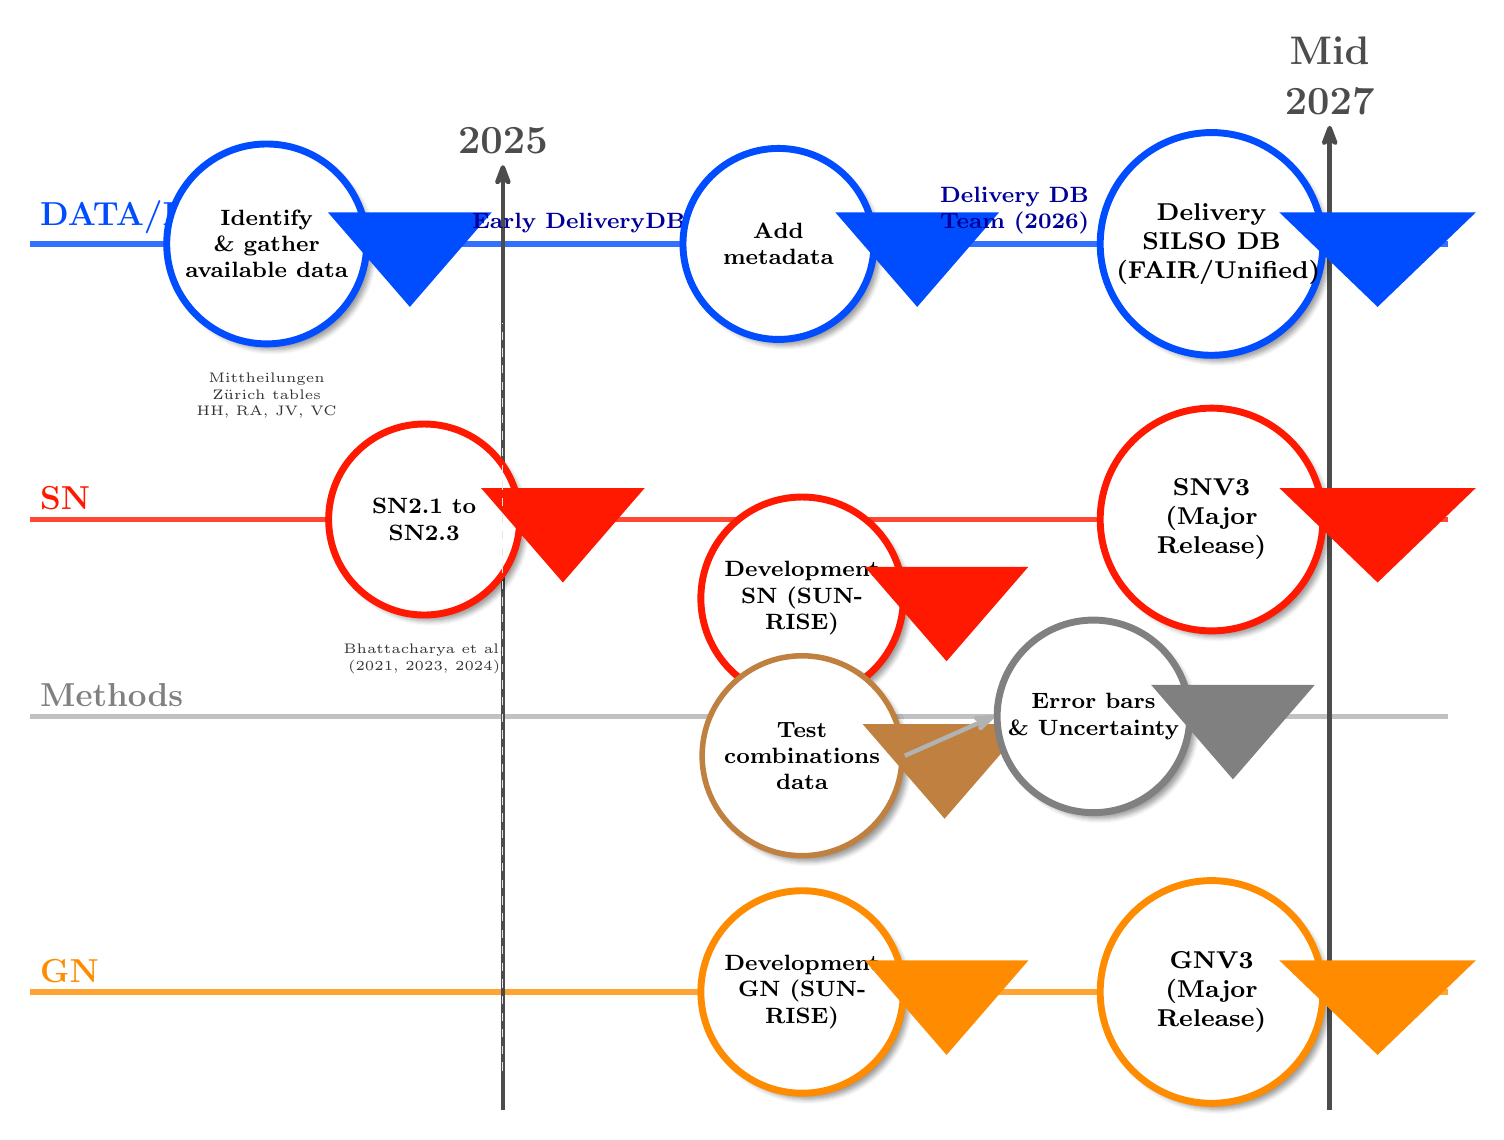
\begin{tikzpicture}[
    % Global Styles
    node distance=1.5cm and 2cm,
    font=\small,
    >={Stealth[round]},
    % Custom Colors based on the image
    colData/.style={draw=blue!70!cyan, fill=white, text=black},
    colSN/.style={draw=red!80!orange, fill=white, text=black},
    colMeth/.style={draw=gray!70, fill=white, text=black},
    colGN/.style={draw=orange!90!yellow, fill=white, text=black},
    % The Bubble Node Style
    bubble/.style 2 args={
        circle,
        draw=#1,
        line width=2.5pt,
        fill=white,
        text width=2.2cm,
        align=center,
        inner sep=2pt,
        font=\footnotesize\bfseries,
        blur shadow={shadow blur steps=5}
    },
    % The "Arrow Tip" attached to bubbles
    pointer/.style={
        fill=#1,
        shape border rotate=270,
        isosceles triangle,
        isosceles triangle apex angle=60,
        inner sep=0,
        minimum height=1.2cm
    },
    % Timeline styling
    timeline/.style={
        line width=2pt,
        opacity=0.8
    }
]

    % --- Grid & Coordinates ---
    % Define horizontal levels
    \coordinate (L1) at (0, 6);   % DATA/DB
    \coordinate (L2) at (0, 2.5); % SN
    \coordinate (L3) at (0, 0);   % Methods
    \coordinate (L4) at (0, -3.5);% GN

    % --- Timelines (Horizontal) ---
    \draw[timeline, blue!70!cyan]    (-2, 6) -- (16, 6) node[right, font=\bfseries\large] {};
    \draw[timeline, red!80!orange]   (-2, 2.5) -- (16, 2.5) node[right, font=\bfseries\large] {};
    \draw[timeline, gray!60]         (-2, 0) -- (16, 0) node[right, font=\bfseries\large] {};
    \draw[timeline, orange!90!yellow](-2, -3.5) -- (16, -3.5) node[right, font=\bfseries\large] {};

    % --- Lane Labels ---
    \node[anchor=south west, text=blue!70!cyan, font=\bfseries\large] at (-2, 6) {DATA/DB};
    \node[anchor=south west, text=red!80!orange, font=\bfseries\large] at (-2, 2.5) {SN};
    \node[anchor=south west, text=gray, font=\bfseries\large] at (-2, 0) {Methods};
    \node[anchor=south west, text=orange!90!yellow, font=\bfseries\large] at (-2, -3.5) {GN};

    % --- Vertical Time Markers ---
    % 2025
    \draw[ultra thick, black!70, ->] (4, -5) -- (4, 7) node[above, font=\bfseries\Large] {2025};
    % Mid 2027
    \draw[ultra thick, black!70, ->] (14.5, -5) -- (14.5, 7.5) node[above, font=\bfseries\Large, align=center] {Mid\\2027};

    % --- STREAM 1: DATA/DB (Blue) ---
    
    % Node 1: Gather Data
    \node[bubble={blue!70!cyan}{}] (db1) at (1, 6) {Identify \& gather available data};
    \node[below=0.2cm of db1, font=\tiny, align=center, text=gray!40!black] {Mittheilungen\\Z\"urich tables\\HH, RA, JV, VC};
    % Pointer 1
    \path (db1.east) ++(-0.2,0) node[pointer, fill=blue!70!cyan, anchor=west, xscale=1.5] {};
    
    % Text on line
    \node[above, font=\footnotesize, text=blue!60!black] at (5.5, 6) {\textbf{Early Delivery}\\\textbf{DB (2025)}};

    % Node 2: Metadata
    \node[bubble={blue!70!cyan}{}] (db2) at (7.5, 6) {Add\\metadata};
    % Pointer 2
    \path (db2.east) ++(-0.2,0) node[pointer, fill=blue!70!cyan, anchor=west, xscale=1.5] {};
    
    % Text on line
    \node[above, font=\footnotesize, text=blue!60!black, align=left] at (10.5, 6) {\textbf{Delivery DB}\\\textbf{Team (2026)}};

    % Node 3: SILSO DB
    \node[bubble={blue!70!cyan}{}, scale=1.1] (db3) at (13, 6) {Delivery\\SILSO DB\\(FAIR/Unified)};
    % Pointer 3
    \path (db3.east) ++(-0.2,0) node[pointer, fill=blue!70!cyan, anchor=west, xscale=1.8] {};


    % --- STREAM 2: SN (Red) ---

    % Node 1: SN2.1
    \node[bubble={red!80!orange}{}] (sn1) at (3, 2.5) {SN2.1 to\\SN2.3};
    \node[below=0.2cm of sn1, font=\tiny, align=center, text=gray!40!black] {Bhattacharya et al.\\(2021, 2023, 2024)};
    % Pointer
    \path (sn1.east) ++(-0.2,0) node[pointer, fill=red!80!orange, anchor=west, xscale=1.5] {};

    % Node 2: Development SN
    \node[bubble={red!80!orange}{}] (sn2) at (7.8, 1.5) {Development\\SN (SUNRISE)};
    % Pointer
    \path (sn2.east) ++(-0.2,0) node[pointer, fill=red!80!orange, anchor=west, xscale=1.5] {};

    % Node 3: SNV3
    \node[bubble={red!80!orange}{}, scale=1.1] (sn3) at (13, 2.5) {\textbf{SNV3}\\(Major Release)};
    % Pointer
    \path (sn3.east) ++(-0.2,0) node[pointer, fill=red!80!orange, anchor=west, xscale=1.8] {};


    % --- STREAM 3: Methods (Gray) ---
    % Note: This stream interacts with SN and GN in the image
    
    % Node 1: Test combinations
    \node[bubble={orange!60!gray}{}, draw=orange!50!gray, line width=2pt] (meth1) at (7.8, -0.5) {Test\\combinations\\data};
    % Pointer
    \path (meth1.east) ++(-0.2,0) node[pointer, fill=orange!50!gray, anchor=west, xscale=1.5] {};
    
    % Node 2: Error bars
    \node[bubble={gray}{}] (meth2) at (11.5, 0) {Error bars\\\& Uncertainty};
    % Pointer
    \path (meth2.east) ++(-0.2,0) node[pointer, fill=gray, anchor=west, xscale=1.5] {};


    % --- STREAM 4: GN (Yellow) ---
    
    % Node 1: Development GN
    \node[bubble={orange!90!yellow}{}] (gn1) at (7.8, -3.5) {Development\\GN (SUNRISE)};
    % Pointer
    \path (gn1.east) ++(-0.2,0) node[pointer, fill=orange!90!yellow, anchor=west, xscale=1.5] {};

    % Node 2: GNV3
    \node[bubble={orange!90!yellow}{}, scale=1.1] (gn2) at (13, -3.5) {\textbf{GNV3}\\(Major Release)};
    % Pointer
    \path (gn2.east) ++(-0.2,0) node[pointer, fill=orange!90!yellow, anchor=west, xscale=1.8] {};


    % --- Manual Adjustments / Decorations ---
    % Connect logic where lines divert in the original image
    
    % Connection from Gray line up to Error Bars
    \draw[ultra thick, gray!60, ->] (meth1.east) -- (meth2.west);
    
    % Dashed vertical lines for alignment visual aid (Optional, kept subtle)
    \draw[dashed, gray!20] (4, -4.5) -- (4, 5);

\end{tikzpicture}

\end{document}
